%%%%%%%%%%%%%%%%%%%%%%%%%%%%%%%%%%%%%%%%%%%%%%%%%%%%%%%%%%
%% BEGIN PREAMBLE
\documentclass[10pt]{article}

%%%% Sets 1 inch margins on document
\usepackage[margin=1in]{geometry}

%%%% For math macros
\usepackage{amsmath}

%%%% Needed for including figures and other images
\usepackage{graphicx}

%%%% Adds ability to adjust document vertical spacing
% usage:
%   \setspace{1.5} % 1.5x for line spacing
\usepackage{setspace}

%%%% Needed for specifying the list items in enumerate env
% eg. (a,b,b) or (i,ii,iii), (1,2,3)
% usage:
%   \begin{enumerate} [label=(\alph*)] % for (a), (b), (c)
\usepackage{enumitem}

%%%% Defines Times New Roman as font
  % for math and text environments
%\usepackage{newtxtext,newtxmath}

  % actually use newcomputermodern
\usepackage{newcomputermodern}

%%%% For H float option when inserting figure
%   [H] inserts figure _exactly_ where it is typeset
% usage:
%   begin{figure} [H]
\usepackage{float}

%%%% For fancy header and footer ;)
\usepackage{fancyhdr}
\pagestyle{fancy}
\fancyhead[LO,L]{Samuel Barton}
\fancyhead[CO,C]{PHYS40 - Homework 6}
\fancyhead[RO,R]{\today}
\fancyfoot[LO,L]{}
\fancyfoot[CO,C]{\thepage}
\fancyfoot[RO,R]{}
\renewcommand{\headrulewidth}{0.4pt}
\renewcommand{\footrulewidth}{0.4pt}

%%%% Setting margins in tabular environments
% For making equations (esp. fractions) fit in cells vertically
\usepackage[column=C]{cellspace}
\cellspacetoplimit 4pt
\cellspacebottomlimit 4pt

%%%% define custom command for a raised chi 
\DeclareRobustCommand{\rchi}{{\mathpalette\irchi\relax}}
\newcommand{\irchi}[2]{\raisebox{\depth}{$#1\chi$}} % inner command, used by \rchi

%%%% For dirac notation
\usepackage{braket}

\usepackage{siunitx}
\DeclareSIUnit\angstrom{Å}

%% END PREAMBLE %%
%%%%%%%%%%%%%%%%%%%%%%%%%%%%%%%%%%%%%%%%%%%%%%%%%%%%%%%%%%%%%%%

\begin{document}

\setstretch{1.25} % set spacing to 1.25x

% Assignment Name
\begin{centering}
  \section*{HOMEWORK 6}
\end{centering}

\begin{enumerate}
\item 
  \begin{enumerate}
  \item 
    The energy for the first ionization of the He atom is 
   \[
     E_1 \approx \frac{2^2E_I}{1^2} = 4 E_I \approx \qty{54.4}{\electronvolt}
   .\]
   The second ionization energy using this approximation is identical, ie,
   \[
     E_2 \approx \qty{54.4}{\electronvolt}
   .\]
  \item
    The discrepancy is most likely due to the electron-electron interactions which are present in this multi-electron atom.
    Since there are multiple electrons, we should not expect the ionization energies to match that of hydrogen, therefore this approximation does not work super well.
    We anticipate that the lower ionization energy is due to the unaccounted repulsion from the coulomb force of the second electron.
    Knowing the true value of the He ground state energy, we have 
    \[
      \qty{79}{\electronvolt} \approx \underbracket{\qty{24.5874}{\electronvolt}}_{\text{Measured}} + \underbracket{\qty{54.4}{\electronvolt}}_{\text{Second Ionization}} = \qty{78.99}{\electronvolt}
    .\]
    The second ionization energy is most likely correct because the He ion only has one electron, and thus behaves like the hydrogen atom.
    Therefore the independent electron approximation works in this case.
  \end{enumerate}
\item
  \begin{enumerate}
  \item
    Each shell can hold $ 2n^2 $ electrons, thus if all six shells were full, we have 
    \[
      \sum_{n=1}^{6} 2n^2 = 2 \left( 1 \right)^2 + 2 \left( 2 \right)^2 + 2 \left( 3 \right)^2 + 2 \left( 4 \right)^2 + 2 \left( 5 \right)^2 + 2 \left( 6 \right)^2 = \qty{182}{elements}
    .\]
  \item
    To verify that the Madelung rule applies (up to 5s), we observe the electron filling pattern:
    \[
      \underbracket{\vphantom{p}1\text{s}}_{1}\underbracket{\vphantom{p}2\text{s}}_{2}\underbracket{2\text{p}}_{3}\underbracket{\vphantom{p}3\text{s}}_{3}\underbracket{3\text{p}}_{4}\underbracket{\vphantom{p}4\text{s}}_{4}\underbracket{\vphantom{p}3\text{d}}_{5}\underbracket{\vphantom{p}5\text{s}}_{5}
    .\]
    Note how subshells fill first in order of increasing $ n+l $, and then within each group, in order of increasing $ n $.
    
    Four exceptions to this rule:
    \begin{enumerate}
    \item Chromium: It should be $ \left[ \text{Ar} \right] 4 \text{s}^2 3 \text{d}^4 $, but it is actually $ \left[ \text{Ar} \right]  4 \text{s}^1 3 \text{d}^5 $
    \item Copper: It should be $ \left[ \text{Ar} \right]  4 \text{s}^2 3 \text{d}^9 $, but it is actually $ \left[ \text{Ar} \right] 4 \text{s}^1 3 \text{d}^{10} $
    \item Niobium: It should be $ \left[ \text{Kr} \right]  5 \text{s}^2 4 \text{d}^3 $, but it is actually $ \left[ \text{Kr} \right] 5 \text{s}^1 3 \text{d}^{4} $
    \item Molybdenum: It should be $ \left[ \text{Kr} \right]  5 \text{s}^2 4 \text{d}^4 $, but it is actually $ \left[ \text{Kr} \right] 5 \text{s}^1 3 \text{d}^{5} $
    \end{enumerate}
  \end{enumerate}
\item
  \begin{enumerate}
  \item
    Using the single electron approximation from question 1, we expect 
    \[
      E_n = \frac{Z_{\text{eff}}E_I}{n^2}
    ,\]
    or,
    \[
      Z_{\text{eff}} = \frac{E_n n^2}{E_I}
    .\]
    Since $ n=3 $ for sodium, we have
    \[
      Z_{\text{eff}} = \frac{E_3 3^2}{E_I} \approx \num{1.84}
    .\]
  \item
    As we move down the alkali metals column in the periodic table, the elements grow larger, and each successive row means an increase in the number of electron shells, or $ n $.
    With the gain of electron shells, we expect that each additional shell adds more "shielding`` to the outermost electrons.
    Thus it makes sense for the ionization energy to decrease as $ n $ grows larger.
  \end{enumerate}
\item
  \begin{enumerate}
  \item See figure:
    \begin{figure} [H]
      \center
      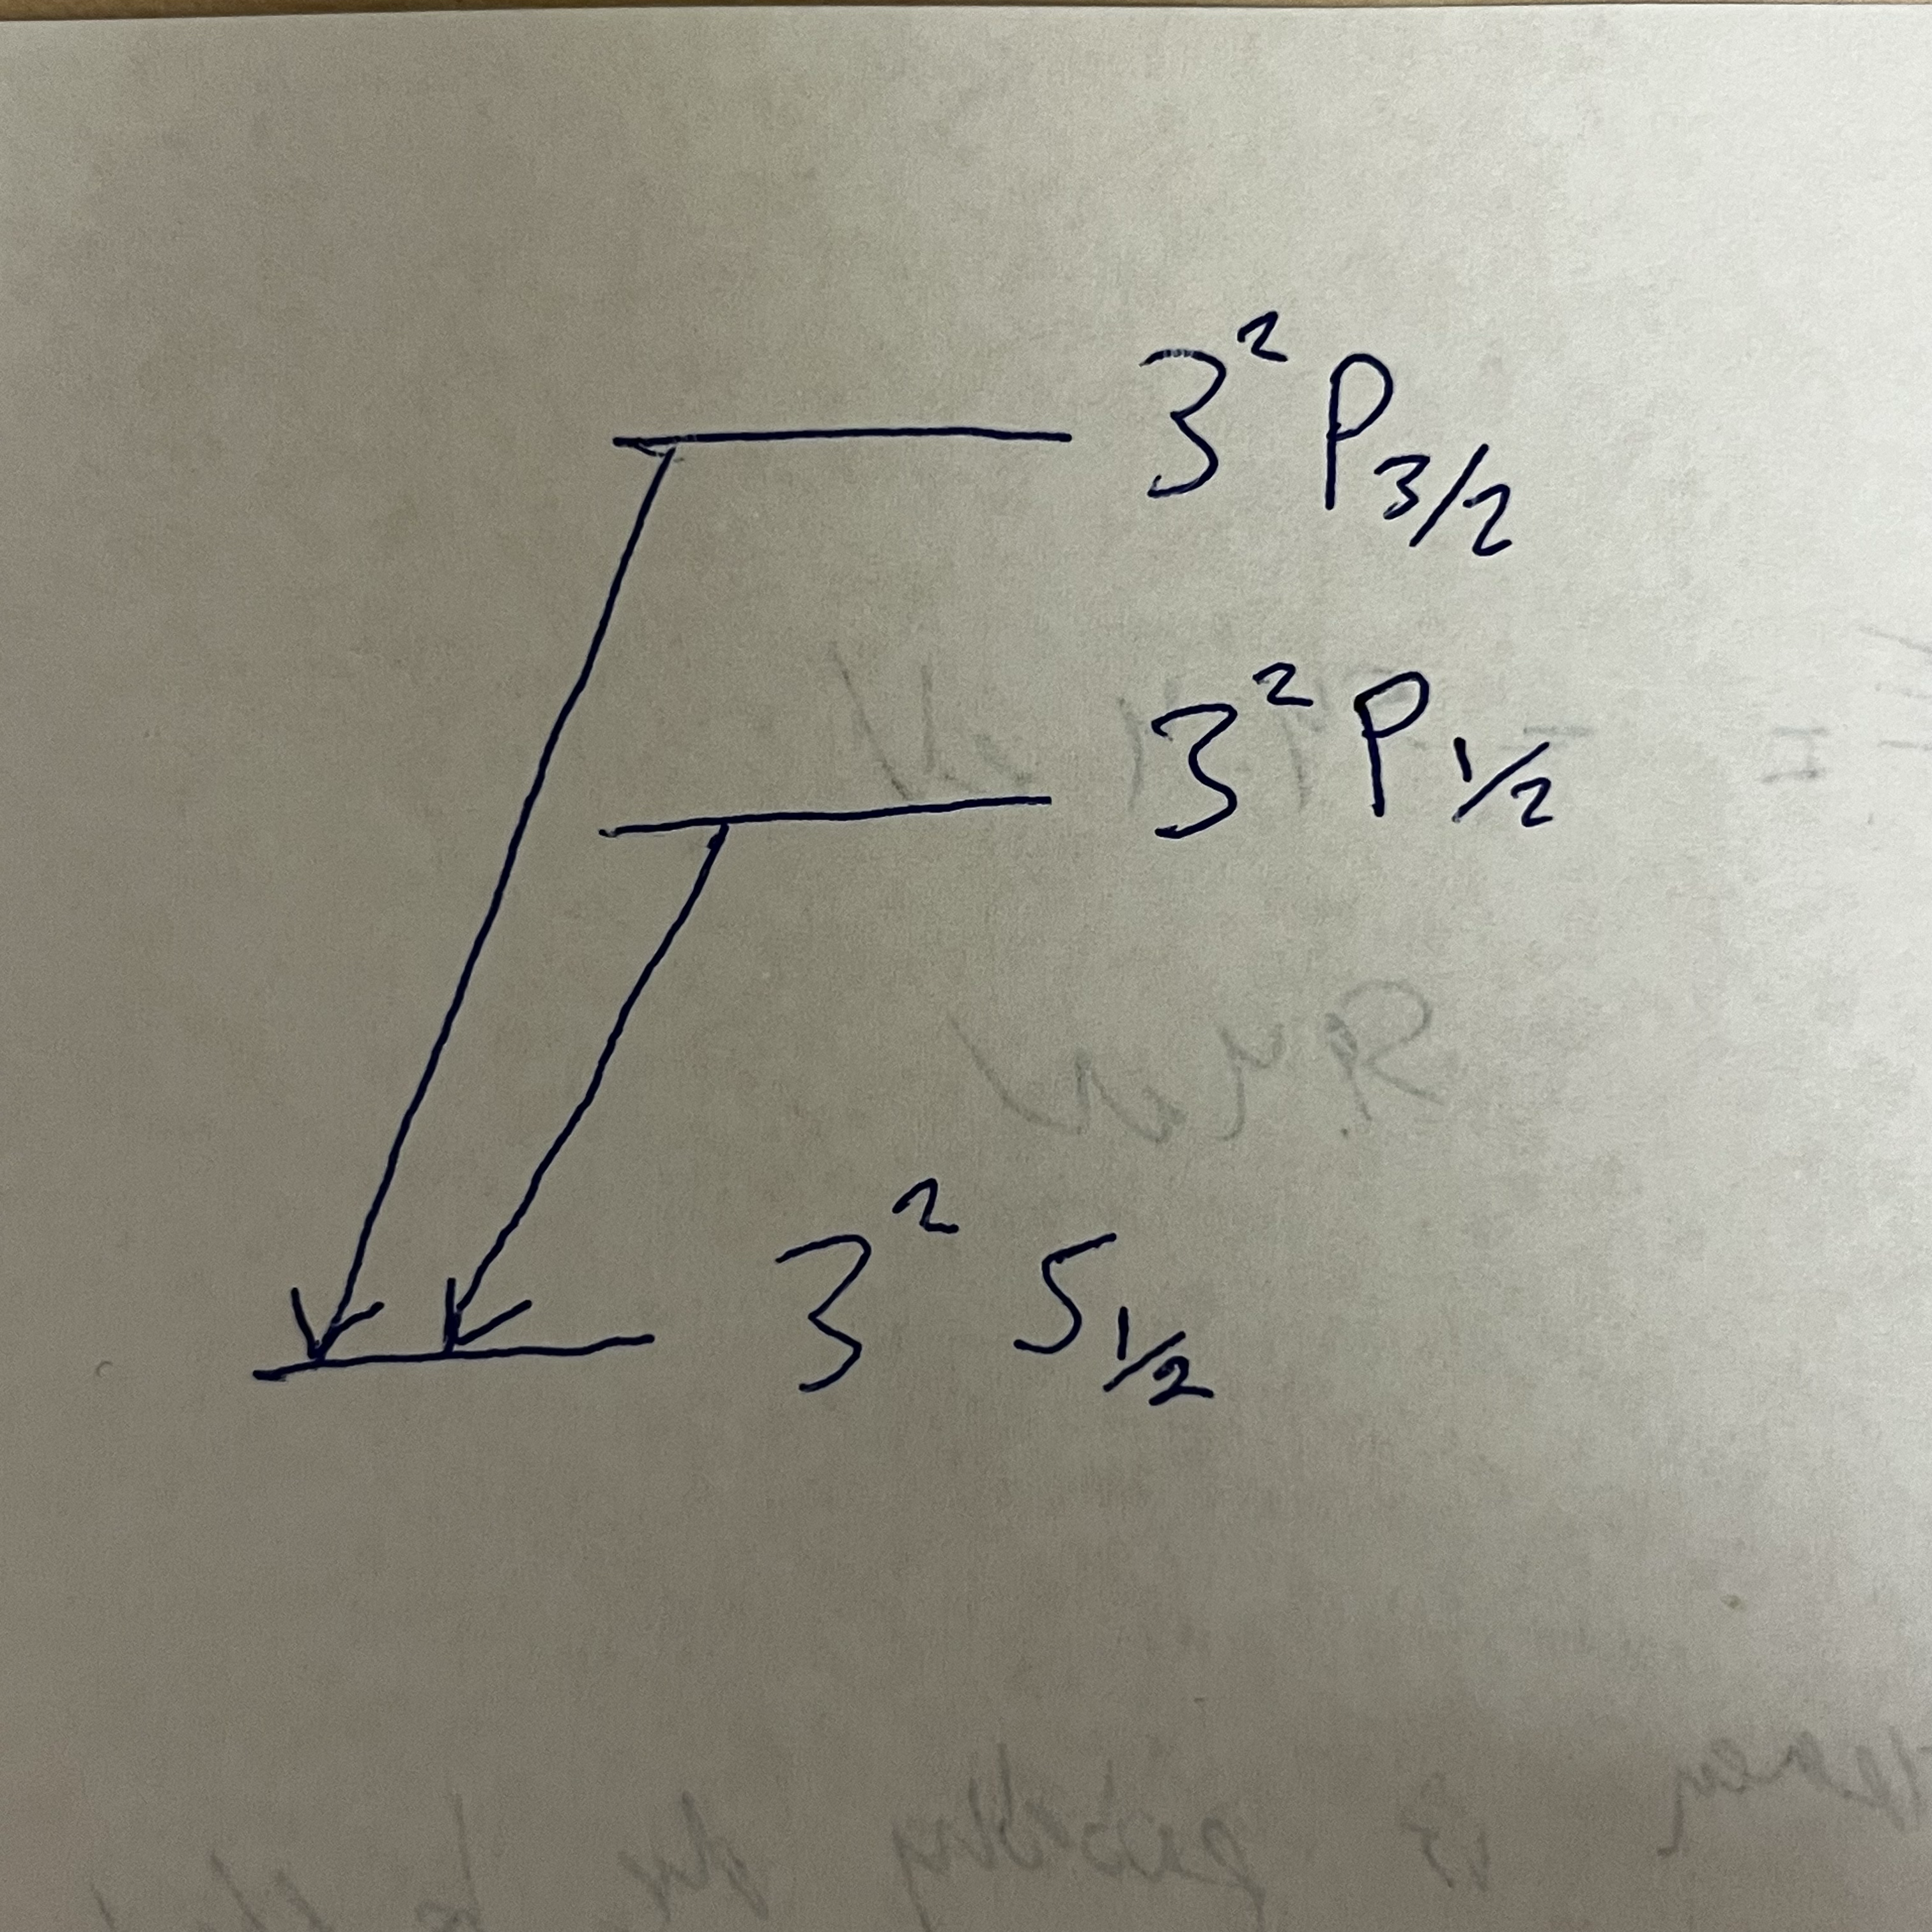
\includegraphics[width=0.6\textwidth]{figures/energy_level_diag.png}
    \end{figure}
  \item
    We have the formula for the change in energy as 
    \[
      \Delta E = \frac{hc}{\lambda_1} - \frac{hc}{\lambda_2} \approx \qty{3.42e-22}{\joule}
    .\]
    For the quantum numbers, we have 
    \begin{align*}
      j=\frac{3}{2},~\frac{1}{2} && l=1 &&& s=\frac{1}{2}
    .\end{align*}
    Thus the equation 
    \[
      \xi \left( L,S \right) = \frac{1}{\Delta E_{SO}} \left[ j\left(j+1\right)-l\left(l+1\right)-s\left(s+1\right) \right]
    \]
    becomes 
    \begin{multline*}
      \Delta E_{SO} \biggl( \left[ \frac{3}{2} \left( \frac{3}{2} + 1 \right) - 1 \left( 1+1 \right) - \frac{1}{2} \left( \frac{1}{2} + 1 \right) \right] \\
      - \left[ \frac{1}{2} \left( \frac{1}{2} + 1 \right) - 1 \left( 1+1 \right) - \frac{1}{2} \left( \frac{1}{2} + 1 \right) \right] \biggr)^{-1} = \frac{\qty{3.42e-22}{\joule}}{3} 
    .\end{multline*}
    Thus, 
    \[
      \xi \left( L,S \right) = \qty{1.14e-22}{\joule}
    \]

    \begin{align*}
      \Delta E &= -\mu_s B \\
               &= g_s \mu B \\
               &=2 \frac{\hslash e}{2m_e}B \\
            B  &= \frac{m_e \Delta E}{\hslash e} \\
            &= \frac{\qty{9.11e-31}{\kg}\cdot \qty{3.42e-22}{\joule} \cdot 2\pi}{\qty{1.6e-19}{\coulomb} \cdot \qty{6.626e-34}{\joule\second}} \\
            &\approx \qty{18.5}{\tesla}
    \end{align*}
  \end{enumerate}
\item
  \begin{enumerate}
  \item
    \begin{gather*}
    \left( 2,~1,~1,~\frac{1}{2},~\frac{1}{2},~0,~\frac{3}{2} \right) \\
    \left( 2,~1,~0,~\frac{1}{2},~\frac{1}{2},~0,~\frac{3}{2} \right) \\
    \left( 2,~1,~-1,~\frac{1}{2},~\frac{1}{2},~0,~\frac{3}{2} \right)
    \end{gather*}
    This state satisfies Pauli Exclusion Principle because no two states have the same exact set of all four quantum numbers.
    This state satisfies Hund's first rule because it has the largest value of $ S $ with all three electrons having spin of $ s=\frac{1}{2} $.
  \item
    Using Hund's first rule, we know that the quartet state, $ ^4S_{3 / 2} $ is the lowest energy state because it has the highest $ S $ value.
    Next, we must use the spin-orbit splitting to order the remaining two states.

    $ ^2D_{3/2} $: $ l=2,\quad s= 1 / 2, \quad j = 3 / 2$
    \[
      \Delta E_{SO} = \xi \left( L,S \right) \left( -3 \right)
    \]
    
    $ ^2P_{3/2} $: $ l=1,\quad s= 1 / 2, \quad j = 3 / 2$
    \[
      \Delta E_{SO} = \xi \left( L,S \right) \left( -2 \right)
    \]

    Thus, we have the final ordering from low to high energy state: $ ^4S_{3 / 2},~ ^2D_{3 / 2},~^2P_{1/2} $.
  \item
    For this state, we see that $ l_1=1,~l_2=1, \text{and}~l_3=0 $. Also, since it is a doublet, $ s= 1 / 2 $.

    The spin states for the $ 2p^2 $ electrons can either be the same, or different.

    First, assume that they are the same, i.e., $ m_{s_1} = 1 / 2,~m_{s_2}=1 / 2,~m_{s_3} = - 1 / 2 $: When listing out possible values for $ m_l $, we see that it must be the case that $ L=1 $. Therefore, $ j=1 / 2,~3 / 2 $. Hence, the spectroscopic notations:
    \[
      ^2P_{1 / 2},~ ^2P_{3 / 2}
    \]
    Next, assume that the spins are different, i.e., $ m_{s_1} = 1 / 2,~m_{s_2}=-1 / 2,~m_{s_3} = - 1 / 2 $. We find that $ L=2 $, and thus $ j = 3 / 2,~5 / 2 $. Hence, the spectroscopic notations:
    \[
      ^2D_{3 / 2},~ ^2D_{5 / 2}
    \]
  \item
    For a quadruplet state, the total spin, $ S=3/2 $, thus the spin for each electron is aligned. If both electrons have the angular momentum quantum number $ l=1 $ to satisfy the total $ L=2 $, then this would violate Pauli's exclusion principle since the two electrons have identical sets of quantum numbers. Therefore, only the doublet state may exist with $ L=2 $, because the spins can be opposite.
  \item
    The second transition rule states that $ \Delta S = 0 $, i.e., there can be no change in total spin. Thus, it is impossible for for a transition between a quartet to a doublet state (or vise versa) since that would violate this rule.
  \item
    The first transition rule states that $ \Delta l_i = \pm 1 $. Therefore, there can be no transitions between the $ 2p $ states since $ \Delta l_i = 0 $ in this case.
  \end{enumerate}
\end{enumerate}

\end{document}

